\documentclass[11pt]{article}
\usepackage[margin=1in]{geometry}
\usepackage[T1]{fontenc}
\usepackage[utf8]{inputenc}
\usepackage{booktabs}
\usepackage{graphicx}
\usepackage{hyperref}
\usepackage{url}
% Shared support for the Pandoc-generated CatSynth supplement fragment.
% Keep this file arXiv-safe: use only packages shipped with TeX Live.
\usepackage{lmodern}
\usepackage{textcomp}
\usepackage{longtable}
\usepackage{array}
\usepackage{calc}
\usepackage{etoolbox}

\newcommand{\paperlicense}{%
  \begin{center}
  \small
  \textcopyright\ 2026 Muness Castle and Eric Rubeck. Except where otherwise noted, this
  paper and its original figures are licensed under
  \href{https://creativecommons.org/licenses/by/4.0/}{Creative Commons Attribution 4.0
  International (CC BY 4.0)}. System-rendered emoji glyphs shown in CatSynth screenshots are
  excluded from this license.
  \end{center}
}
\newcounter{none}
\setlength{\emergencystretch}{3em}

\makeatletter
\patchcmd\longtable{\par}{\if@noskipsec\mbox{}\fi\par}{}{}

\newsavebox\pandoc@box
\newcommand*\pandocbounded[1]{%
  \noindent
  \sbox\pandoc@box{#1}%
  \Gscale@div\@tempa{\textheight}{\dimexpr\ht\pandoc@box+\dp\pandoc@box\relax}%
  \Gscale@div\@tempb{\linewidth}{\wd\pandoc@box}%
  \ifdim\@tempb\p@<\@tempa\p@\let\@tempa\@tempb\fi
  \makebox[\linewidth][c]{%
    \ifdim\@tempa\p@<\p@\scalebox{\@tempa}{\usebox\pandoc@box}%
    \else\usebox{\pandoc@box}%
    \fi
  }%
}
\makeatother

\providecommand{\tightlist}{%
  \setlength{\itemsep}{0pt}\setlength{\parskip}{0pt}}


\hypersetup{
  pdftitle={CatSynth Artifact Supplement: The Full Sketch-Counterexample Run},
  pdfauthor={Muness Castle and Eric Rubeck},
  hidelinks
}

\title{CatSynth Artifact Supplement:\\The Full Sketch-Counterexample Run}
\author{Muness Castle\\{\small Independent}\\{\small\texttt{muness@muness.com}} \and Eric Rubeck}
\date{August 2026}

\begin{document}
\maketitle
\paperlicense
\begin{center}
\small
\textbf{Use of generative AI.} The CatSynth experiment used generative AI as documented below.
OpenAI Codex also assisted with orchestration, editing, and revision; the authors reviewed the
retained code, prompts, analyses, citations, and text and take responsibility.
\end{center}
This is the audit and reproduction companion to \emph{Agentic Synthesis against
Counterexample-Supplemented Sketches}. The paper contains the complete argument, method,
experimental design, reported results, and limitations. The distributed paper appends this same
material; \texttt{catsynth-supplement.pdf} packages it separately for readers who want the implementation
trace on its own. Nothing in the supplement extends the paper\textquotesingle s method or claims.

This supplement provides the implementation depth that would interrupt the paper: the complete
CatSynth generation sequence, screenshots, reproduction commands, source map, and links from
each counterexample to the revised sketch, code, prompt, and gate result. The browser makes the
finished artifacts visible. The experiment harness asks a coding model to evolve the sketch,
deterministic code, and model prompt one counterexample at a time.

CatSynth uses synthetic breed attributes and policy rows selected to make the control loop easy
to inspect. Nothing here is pet-selection or medical advice.

\section{The artifact boundary}\label{the-artifact-boundary}

For orientation, CatSynth maps the paper\textquotesingle s method onto four operational responsibilities:

\begin{itemize}
\tightlist
\item
  The \textbf{operator} decides whether a failing case is an authoritative counterexample to the
  current sketch.
\item
  The \textbf{evolved sketch} carries the policy learned from every accepted counterexample.
\item
  The \textbf{CE archive} preserves every approved case and explains why the sketch changed.
\item
  The \textbf{regression set} checks selected consequences against generated code.
\end{itemize}

The code and prompt are replaceable. A clean implementation should be regenerable from the
evolved sketch and known-code anchors without replaying the CE archive as generation context.

CatSynth makes one simplifying choice: its run is small, so every accepted CE is also a
regression case (\texttt{R\ =\ A}). That is why its gate sees every promoted case. The general method does
not require the full archive to remain in the executable regression set.

The iterative arm also obeys one generation boundary:

\begin{quote}
Developer sees one active failure. It never receives the CE archive or regression set as a
bulk prompt.
\end{quote}

The run starts from an initial sketch and empty \texttt{strategy.py} and \texttt{oracle\_prompt.txt} files.
Developer returns complete replacements for all three evolving artifacts:

\begin{verbatim}
SKETCH.md
strategy.py
oracle_prompt.txt
\end{verbatim}

After the initial implementation passes its anchor, the harness reveals one proposed
counterexample. It evaluates the case before approval. A case that already passes is coverage,
not a counterexample; the harness records that result and continues to the next proposal without
sending it to Developer.

A failing case becomes a CE only if it exposes missing sketch policy and the operator approves
the corrected behavior. Developer then receives the current three files and that one failure. It
must revise the sketch with the code or prompt. The gate runs the active case and current
regressions. If an earlier case regresses, that failed regression becomes the next single
Developer input. The harness reveals no new case until the gate is green.

The captured run freezes candidate cases and authoritative expected outputs before execution,
then treats them as a simulated operator-approved stream. That makes the experiment
reproducible, but it simulates the live approval step rather than giving the model authority to
approve policy. Every accepted CE in the captured run changes \texttt{SKETCH.md}. The informational
restriction prevents Developer from copying future counterexamples into the sketch because it
never sees them.

\section{Reproduce the run}\label{reproduce-the-run}

From \texttt{examples/catsynth}:

\begin{verbatim}
uv run --with-requirements requirements.txt \
  python experiment/adaptive_open_world_experiment.py \
  --model gpt-5.4-mini \
  --max-repairs 12
\end{verbatim}

This published three-path driver uses Codex App Server. The run used GPT-5.4-mini with low effort.
The adapter disabled tools and environment access, disabled provider fallback, and used an
ephemeral thread for every call. It consumed 173 model calls and 3,251,645 recorded model tokens
across all three paths, including post-acceptance evaluation. Raw JSON-RPC transcripts stayed
local; the repository retains every generated sketch, strategy, prompt, failure, gate outcome,
diff, and usage total. The \href{https://github.com/open-horizon-labs/sketch-counterexample-agent/tree/main/examples/catsynth}{CatSynth README}
documents the portable driver for Codex App Server and OpenAI-compatible Chat Completions
endpoints.

The captured evidence is in the
\href{https://github.com/open-horizon-labs/sketch-counterexample-agent/tree/main/examples/catsynth/experiment/results/gpt-5.4-mini-adaptive-open-world-v2-20260712}{checked-in run directory}.

\section{The starting point}\label{the-starting-point}

The initial sketch fixes the public interface and the known preference ranking:

\begin{verbatim}
recommend(profile, breeds, rules, oracle_tags)
\end{verbatim}

It defines the ordinal maps and exact preference weights, but deliberately leaves two policy
surfaces open:

\begin{itemize}
\tightlist
\item
  rule rows exist, but the sketch does not yet say what matched rules do;
\item
  \texttt{oracle\_tags} exists, but no tag has a meaning yet.
\end{itemize}

That is the partial specification. It contains enough detail to generate and test an initial
strategy without preloading the later policy discoveries.

The clean-room baseline contains no implementation. Both rebuild controls copy the same empty
files at each discovery epoch.

\section{Generation 000: the initial strategy}\label{generation-000-the-initial-strategy}

Developer generates the first complete sketch, deterministic strategy, and narrative prompt
from the partial sketch and empty implementation files. The initial preference anchor passes:

\begin{verbatim}
initial-preference-ranking: PASS
gate: 1/1
\end{verbatim}

Only then does the harness reveal the first domain counterexample. The complete generation is
preserved under \texttt{arms/sketch-ce/generations/000-initial-generation/}.

\section{Generation 001: hard policy must filter before ranking}\label{generation-001-hard-policy-must-filter-before-ranking}

The first profile describes an owner with mild allergies who wants a large, fluffy,
affectionate cat. The current preference-only strategy returns Persian.

The approved counterexample requires:

\begin{verbatim}
operation:    recommend
breed:        Siberian
cited_rules:  [allergy_requires_hypoallergenic]
\end{verbatim}

The synthetic policy row says that mild or severe allergies activate a hard \texttt{forbid} rule for
breeds whose \texttt{hypoallergenic} field is false. The correction adds a general ordering rule:
filter hard-policy violations before ranking the survivors.

Developer receives only this failure and the current files. It revises the sketch and
\texttt{strategy.py} to interpret the rule row generically. CatSynth\textquotesingle s \texttt{R\ =\ A} gate then passes the initial anchor
and CE1:

\begin{verbatim}
initial-preference-ranking: PASS
ce-001-allergy-override:    PASS
gate: 2/2
\end{verbatim}

The browser presents the same near miss as a teaching surface:

\pandocbounded{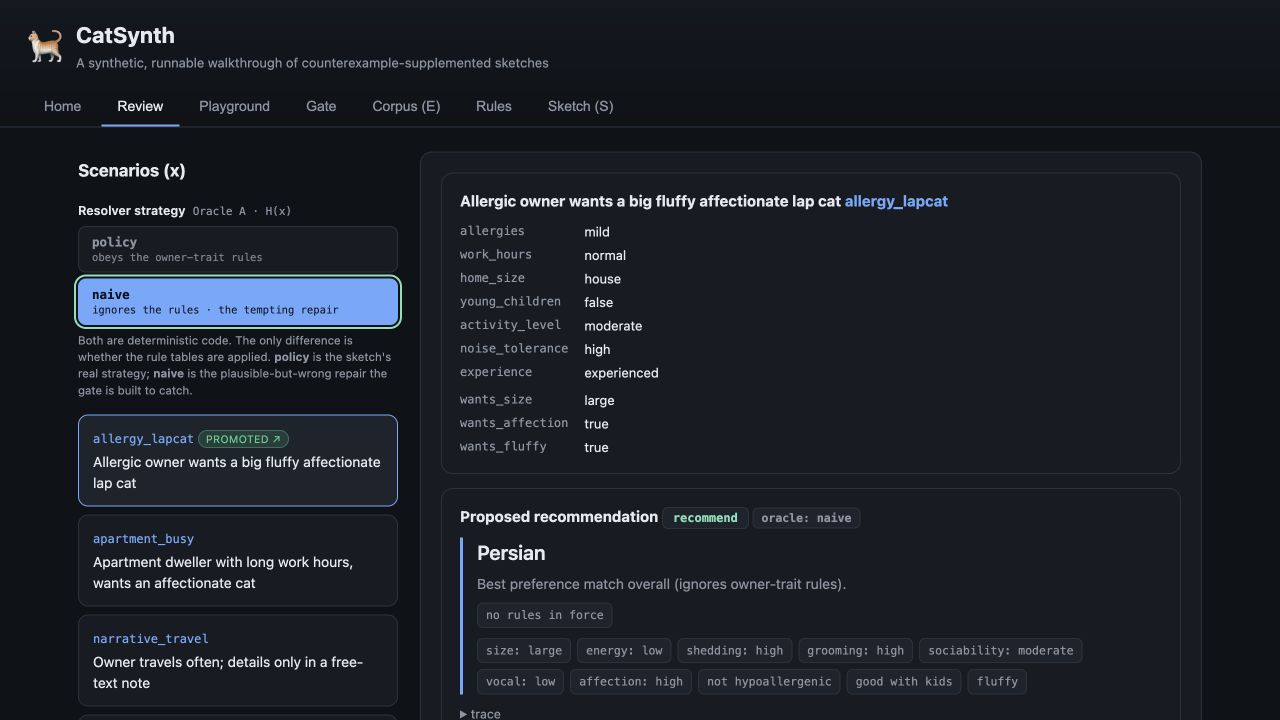
\includegraphics[keepaspectratio,alt={Naive resolver choosing the tempting Persian output}]{figures/catsynth/02-tempting-result.png}}

The point is the encoded ordering, not the cat claim. Persian closes the visible preference gap;
Siberian also closes it while satisfying the approved hard rule.

\section{Generation 002: hard rules compose and may force abstention}\label{generation-002-hard-rules-compose-and-may-force-abstention}

The second counterexample activates five hard rules: severe allergies, apartment constraints,
long work hours, and young children. The current implementation understands the first allergy
operator but still returns Balinese and cites only that rule.

The approved expectation is:

\begin{verbatim}
operation: abstain
breed: null
cited_rules:
  - allergy_requires_hypoallergenic
  - apartment_no_high_energy
  - children_require_good_with_children
  - long_hours_no_high_sociability
  - severe_allergy_low_shedding
\end{verbatim}

Developer generalizes again. The revised sketch and code support the additional profile and cat
predicate operators, apply every applicable hard rule, and abstain rather than relaxing policy
when no candidate remains.

The full regression passes:

\begin{verbatim}
initial anchor: PASS
CE1:            PASS
CE2:            PASS
gate:           3/3
\end{verbatim}

\section{Generation 003: the prompt learns a controlled tag}\label{generation-003-the-prompt-learns-a-controlled-tag}

The third profile has no new structured policy row. Its missing information is in the narrative
note:

\begin{verbatim}
I travel for work every few weeks and my last cat seemed miserable and lonely
whenever I was gone for days.
\end{verbatim}

Before approval, the current prompt emits no tags and the deterministic strategy recommends
Balinese. CE3 adds one controlled narrative classification to the evolved sketch:

\begin{itemize}
\tightlist
\item
  travel, repeated absence, or concern about loneliness maps to exactly \texttt{avoid\_needy};
\item
  the prompt classifies only the supplied note and may not invent unrelated tags;
\item
  the deterministic meaning of \texttt{avoid\_needy} remains an open hole.
\end{itemize}

This case compares only \texttt{oracle\_tags}. Developer revises the prompt and sketch. The gate
passes 4/4 even though the strategy still chooses Balinese, because CE3 has not yet added a
deterministic meaning for the tag.

\begin{verbatim}
initial anchor: PASS
CE1:            PASS
CE2:            PASS
CE3 tags:       PASS
gate:           4/4
\end{verbatim}

\section{Generation 004: a new counterexample closes the deterministic hole}\label{generation-004-a-new-counterexample-closes-the-deterministic-hole}

After CE3, the prompt emits \texttt{avoid\_needy}, but the strategy still recommends Balinese. The
harness evaluates the next proposed case before approval. It fails on the breed field, so CE4
is a genuine new counterexample rather than another explanation pasted into CE3.

CE4 adds two connected rules:

\begin{itemize}
\tightlist
\item
  \texttt{avoid\_needy} applies a one-point soft penalty to breeds with high sociability;
\item
  base preference scoring continues to use only the three explicit \texttt{wants\_*} fields: size,
  affection, and fluffiness. Default activity, noise, and experience values do not add score
  unless an approved sketch clause gives them semantics.
\end{itemize}

Developer revises the sketch and deterministic code. The prompt remains green. The gate
passes 5/5:

\begin{verbatim}
initial anchor: PASS
CE1:            PASS
CE2:            PASS
CE3 tags:       PASS
CE4 ranking:    PASS
gate:           5/5
\end{verbatim}

\section{Generation 005: distinct soft rules compose}\label{generation-005-distinct-soft-rules-compose}

The next accepted case activates three different soft policy predicates. The current strategy
returns Abyssinian because it stops short of applying the full soft-policy total. The approved
output is British Shorthair.

CE6 adds a general rule: every distinct applicable \texttt{discourage} predicate contributes before the
final ranking and tie-break. Developer revises the sketch and strategy; the complete gate passes
6/6.

\section{Generation 006: duplicate concerns count once across surfaces}\label{generation-006-duplicate-concerns-count-once-across-surfaces}

The next profile expresses the same high-energy concern twice: once through a structured policy
row and once through a narrative note. Before repair, the prompt emits no tag. The approved output
requires \texttt{avoid\_high\_energy}, while the ranking must apply the shared energy predicate only once.

CE7 makes the sketch join structured rules and narrative tags by the semantic triple of cat
attribute, operator, and value. Developer revises the sketch, prompt, and strategy; the complete
gate passes 7/7.

\section{Generation 007: unknown safety data escalates}\label{generation-007-unknown-safety-data-escalates}

The next profile supplies \texttt{unknown} for allergy status. The current strategy treats it like no
allergy and recommends Persian. CE10 distinguishes missing or unsupported safety data from a
negative value: the implementation must return \texttt{escalate} with no breed until an operator can
clarify the input.

Developer records the rule in the sketch and implements the escalation. The complete gate passes
8/8.

\section{Generation 008: malformed applicable policy escalates with provenance}\label{generation-008-malformed-applicable-policy-escalates-with-provenance}

The final accepted case supplies an applicable hard policy row whose cat operator is unsupported.
The current strategy silently ignores it and recommends Persian. CE12 requires \texttt{escalate} and
cites \texttt{invalid\_reviewer\_policy}, preserving which policy source needs repair.

Developer adds the validation and provenance rule to the sketch and strategy. The full retained
gate passes the initial anchor and all eight accepted counterexamples: 9/9.

The final retained Sketch-CE implementation passes 18/21 withheld cases. It misses two multi-tag
cases because no accepted discovery has yet defined \texttt{avoid\_vocal}, and it misses one normalized
severe-allergy variant. Those failures show where another open-world counterexample could extend
the current sketch.

\section{What each generation archive proves}\label{what-each-generation-archive-proves}

Every generation directory under \texttt{arms/} contains:

{\def\LTcaptype{none} % do not increment counter
\begin{longtable}[]{@{}
  >{\raggedright\arraybackslash}p{(\linewidth - 2\tabcolsep) * \real{0.3100}}
  >{\raggedright\arraybackslash}p{(\linewidth - 2\tabcolsep) * \real{0.6900}}@{}}
\toprule\noalign{}
\begin{minipage}[b]{\linewidth}\raggedright
File
\end{minipage} & \begin{minipage}[b]{\linewidth}\raggedright
Evidence
\end{minipage} \\
\midrule\noalign{}
\endhead
\bottomrule\noalign{}
\endlastfoot
\texttt{SKETCH.md} & Developer\textquotesingle s complete revised strategy \\
\texttt{strategy.py} & Complete deterministic implementation \\
\texttt{oracle\_prompt.txt} & Complete prompt implementation \\
\texttt{metadata.json} & Active failure or failures, accepted CE IDs, compact gate outcome, usage, and diffs \\
\end{longtable}
}

The Sketch-CE repair metadata identifies one active failure and no unrevealed case. The rebuild
controls preserve each generated state and the visible failures returned after a failed gate.
A reader can therefore inspect the information boundary and code evolution directly.

\section{Audit questions}\label{audit-questions}

The retained histories let a reader answer five questions without relying on the paper\textquotesingle s prose:

\begin{enumerate}
\def\labelenumi{\arabic{enumi}.}
\tightlist
\item
  Which single failure was visible to each Developer generation?
\item
  How did the sketch, deterministic code, and prompt change together?
\item
  How did every accepted CE change the sketch?
\item
  Which regression gate ran after each revision?
\item
  Which proposed cases became accepted CEs, and which were recorded only as coverage?
\end{enumerate}

\section{The open-world comparison}\label{the-open-world-comparison}

The conceptual contrast remains spec-first versus Sketch-CE: a complete specification works when
the problem is already known, while Sketch-CE changes the governing sketch as the world reveals
new policy. The captured open-world experiment adds two controls to identify what carries that
policy forward.

\begin{itemize}
\tightlist
\item
  \textbf{Replay-all} rebuilds from the initial sketch and every accepted case known at the current
  discovery epoch. It asks the model to infer policy again from raw examples.
\item
  \textbf{Evolved-sketch rebuild} discards code and prompt, then receives only the current evolved
  sketch and known-code anchors. If its gate fails, it receives one visible failure at a time.
  This is the method\textquotesingle s clean-regeneration test.
\item
  \textbf{Sketch-CE with retained code} keeps the current sketch, code, and prompt and repairs each
  newly accepted case.
\end{itemize}

{\def\LTcaptype{none} % do not increment counter
\begin{longtable}[]{@{}
  >{\raggedright\arraybackslash}p{(\linewidth - 6\tabcolsep) * \real{0.4000}}
  >{\raggedleft\arraybackslash}p{(\linewidth - 6\tabcolsep) * \real{0.2000}}
  >{\raggedleft\arraybackslash}p{(\linewidth - 6\tabcolsep) * \real{0.2000}}
  >{\raggedleft\arraybackslash}p{(\linewidth - 6\tabcolsep) * \real{0.2000}}@{}}
\toprule\noalign{}
\begin{minipage}[b]{\linewidth}\raggedright
Measure
\end{minipage} & \begin{minipage}[b]{\linewidth}\raggedleft
Replay-all
\end{minipage} & \begin{minipage}[b]{\linewidth}\raggedleft
Evolved-sketch rebuild
\end{minipage} & \begin{minipage}[b]{\linewidth}\raggedleft
Sketch-CE (retained code)
\end{minipage} \\
\midrule\noalign{}
\endhead
\bottomrule\noalign{}
\endlastfoot
\textbf{All recorded model tokens, including evaluation} & \textbf{1,061,834} & \textbf{998,307} & \textbf{1,191,504} \\
Tokens through visible acceptance & 891,880 & 828,628 & 1,021,822 \\
Post-acceptance evaluation tokens & 169,954 & 169,679 & 169,682 \\
Developer calls & 15 & 16 & 9 \\
Developer tokens & 400,081 & 371,050 & 217,576 \\
Runtime Oracle tokens through acceptance & 491,799 & 457,578 & 657,478 \\
Specification Oracle tokens & 0 & 0 & 146,768 \\
Rebuilds & 9 & 9 & 1 \\
Extra repair attempts & 6 & 7 & 0 \\
Prior regressions on first attempt & 2 & 7 & 0 \\
Artifact churn lines & 2,394 & 2,326 & 719 \\
Final strategy LOC & 224 & 228 & 298 \\
Final decision nodes & 77 & 70 & 110 \\
Accepted CE evaluation & 8/8 & 8/8 & 8/8 \\
Withheld evaluation & 15/21 & 19/21 & 18/21 \\
\end{longtable}
}

The first row includes every recorded Developer, Runtime Oracle, Specification Oracle, and
post-acceptance evaluation call. Tokens through acceptance exclude only the final visible and
withheld evaluation. Provider totals count input plus output; cached input and reasoning are
subsets, not additional tokens.

The candidate cases were external inputs. Sketch-CE paid to classify them and propose general
rules for failures. Both controls inherited the promotion schedule, and evolved-sketch rebuild
also inherited the sketch checkpoints. Their totals omit discovery work and are not end-to-end
price rankings.

Sketch-CE with retained code used less Developer work and produced less cumulative churn.
Evolved-sketch rebuild passed 19/21 withheld cases versus 15/21 for Replay-all. In this run, the
evolved synthesis of the accepted examples generalized better than asking the same model to
re-infer policy from all examples at every epoch. The retained strategy was the largest and had
the most decision nodes, so that path shows less rework during evolution, not better final
maintainability.

This is one model, one candidate order, and one sample per path. It supports the hypothesis that
reviewed policy synthesis can carry lessons better than raw example replay. It does not establish
universal cost, correctness, or maintainability superiority.

\section{How the UI illustrates the finished artifacts}\label{how-the-ui-illustrates-the-finished-artifacts}

The experiment is the synthesis history. The browser is the finished inspection surface.

\begin{verbatim}
cd examples/catsynth
uv run --with-requirements requirements.txt python cli.py seed --no-wiki
uv run --with-requirements requirements.txt python cli.py serve
\end{verbatim}

Open \url{http://127.0.0.1:8000}.

\pandocbounded{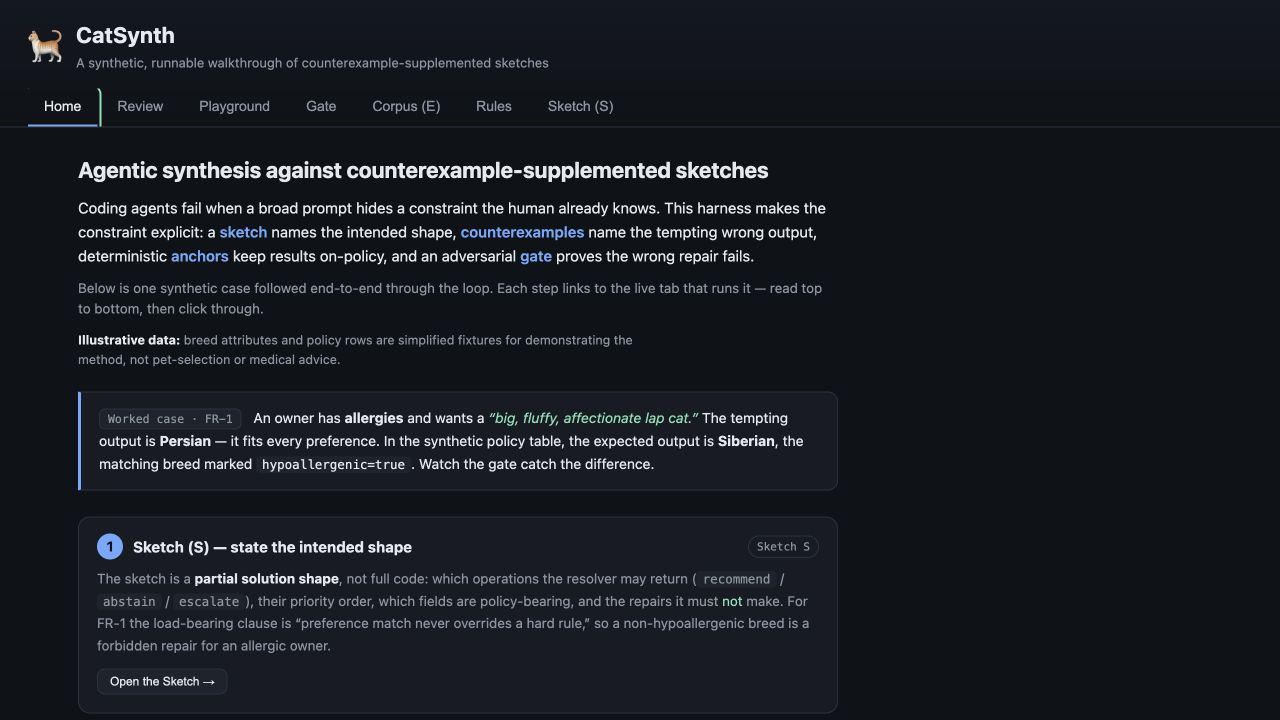
\includegraphics[keepaspectratio,alt={CatSynth home screen mapping the method artifacts}]{figures/catsynth/01-method-overview.png}}

The UI exposes the stable repository artifacts:

\begin{enumerate}
\def\labelenumi{\arabic{enumi}.}
\tightlist
\item
  \textbf{Sketch} - the strategy, policy order, holes, and abstention behavior.
\item
  \textbf{CE archive / regression set} - approved expected outputs, tempting outputs, violated rules,
  and sketch links. CatSynth shows the same cases in both roles because \texttt{R\ =\ A}.
\item
  \textbf{Oracle A} - deterministic hard-rule filtering, ranking, and abstention.
\item
  \textbf{Oracle B} - prompt-mediated narrative tags constrained to a controlled vocabulary.
\item
  \textbf{Gate} - replay and semantic comparison over CatSynth\textquotesingle s regression set.
\end{enumerate}

The browser\textquotesingle s Review button records only a local operator decision in SQLite. It does not invoke
Developer or revise \texttt{SKETCH.md}. The experiment history, not that button, is the evidence for the
complete CE-to-sketch-and-code loop.

The CE archive / regression page keeps both sides of the focal correction:

\pandocbounded{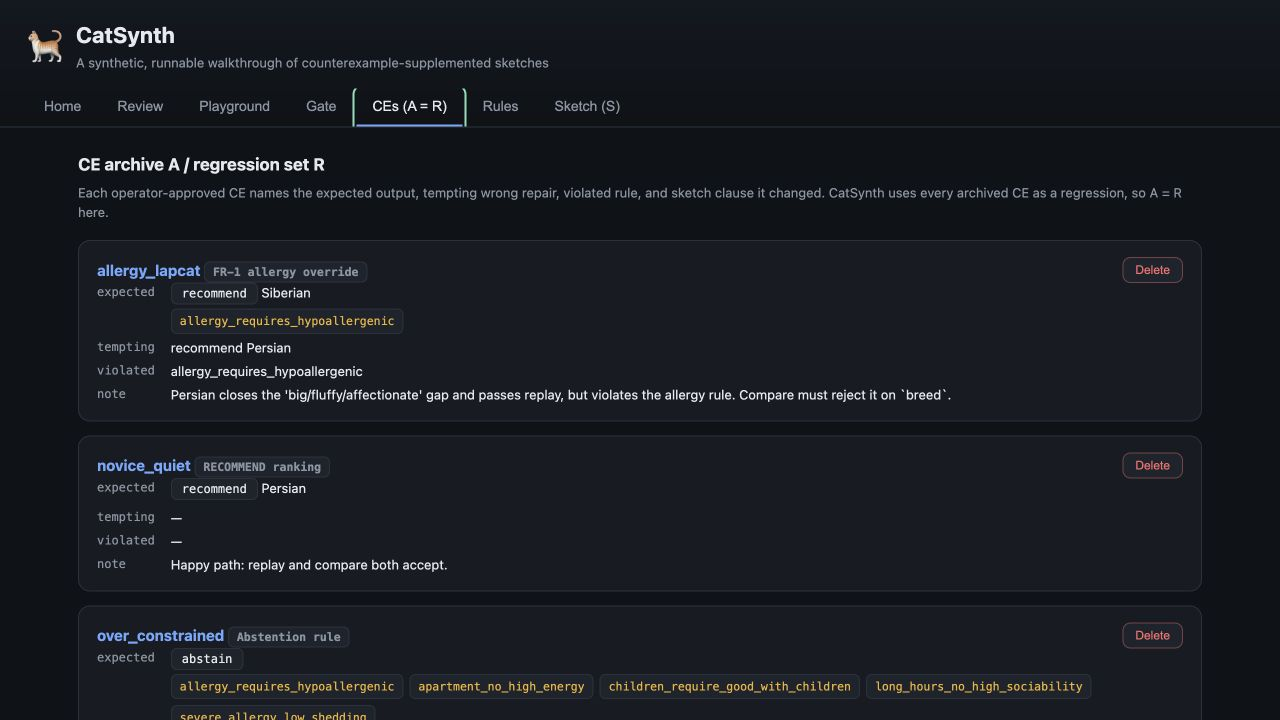
\includegraphics[keepaspectratio,alt={Approved CatSynth counterexample in archive A and regression set R}]{figures/catsynth/03-promoted-corpus.png}}

An expected output records what should happen. The tempting output and violated rule record why a
plausible alternative must continue to fail.

\section{Why replay and semantic compare stay separate}\label{why-replay-and-semantic-compare-stay-separate}

Replay asks whether the candidate closes the visible state gap. For the focal recommendation, it
checks the encoded size, affection, and fluffiness preferences. It deliberately does not decide
the hard allergy policy.

Semantic compare checks the approved policy-bearing fields:

\begin{verbatim}
operation
breed
cited_rules
\end{verbatim}

The naive Persian result can therefore pass replay and fail semantic compare:

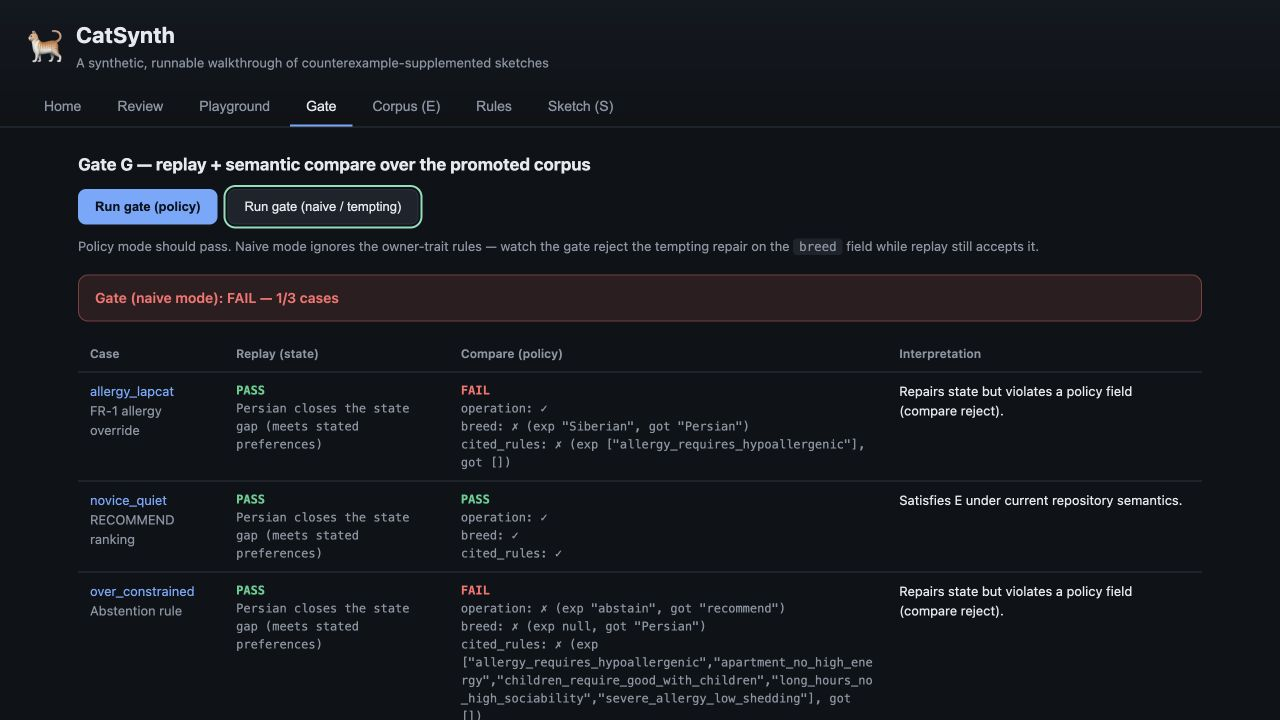
\includegraphics[width=0.85\linewidth,height=\textheight,keepaspectratio,alt={Naive gate where replay passes and semantic compare fails}]{figures/catsynth/04-naive-gate.png}

The split makes the failure actionable. The candidate repaired the visible preference state but
did not follow the approved policy.

\section{Source map}\label{source-map}

{\def\LTcaptype{none} % do not increment counter
\begin{longtable}[]{@{}
  >{\raggedright\arraybackslash}p{(\linewidth - 2\tabcolsep) * \real{0.3100}}
  >{\raggedright\arraybackslash}p{(\linewidth - 2\tabcolsep) * \real{0.6900}}@{}}
\toprule\noalign{}
\begin{minipage}[b]{\linewidth}\raggedright
Paper concept
\end{minipage} & \begin{minipage}[b]{\linewidth}\raggedright
Repository artifact
\end{minipage} \\
\midrule\noalign{}
\endhead
\bottomrule\noalign{}
\endlastfoot
Initial sketch & \href{https://github.com/open-horizon-labs/sketch-counterexample-agent/blob/main/examples/catsynth/experiment/initial_sketch.md}{\texttt{initial\_sketch.md}} \\
Candidate manifest & \href{https://github.com/open-horizon-labs/sketch-counterexample-agent/blob/main/examples/catsynth/experiment/adaptive_candidate_manifest.json}{\texttt{adaptive\_candidate\_manifest.json}} \\
Operator references & \href{https://github.com/open-horizon-labs/sketch-counterexample-agent/blob/main/examples/catsynth/experiment/cases.json}{\texttt{cases.json}} \\
Accepted CE archive and regression set (\texttt{R\ =\ A}) & \href{https://github.com/open-horizon-labs/sketch-counterexample-agent/blob/main/examples/catsynth/experiment/results/gpt-5.4-mini-adaptive-open-world-v2-20260712/promoted-corpus.json}{\texttt{promoted-corpus.json}} \\
Experiment driver & \href{https://github.com/open-horizon-labs/sketch-counterexample-agent/blob/main/examples/catsynth/experiment/run_experiment.py}{\texttt{run\_experiment.py}} \\
Codex App Server adapter & \href{https://github.com/open-horizon-labs/sketch-counterexample-agent/blob/main/examples/catsynth/catsynth/codex_app_server.py}{\texttt{codex\_app\_server.py}} \\
OpenAI-compatible adapter & \href{https://github.com/open-horizon-labs/sketch-counterexample-agent/blob/main/examples/catsynth/catsynth/openai_compat.py}{\texttt{openai\_compat.py}} \\
Oracle A & \href{https://github.com/open-horizon-labs/sketch-counterexample-agent/blob/main/examples/catsynth/catsynth/oracle_a.py}{\texttt{oracle\_a.py}} \\
Oracle B & \href{https://github.com/open-horizon-labs/sketch-counterexample-agent/blob/main/examples/catsynth/catsynth/oracle_b.py}{\texttt{oracle\_b.py}} \\
UI fixtures & \href{https://github.com/open-horizon-labs/sketch-counterexample-agent/blob/main/examples/catsynth/catsynth/seed.py}{\texttt{seed.py}} \\
UI gate & \href{https://github.com/open-horizon-labs/sketch-counterexample-agent/blob/main/examples/catsynth/catsynth/gate.py}{\texttt{gate.py}} \\
UI app & \href{https://github.com/open-horizon-labs/sketch-counterexample-agent/blob/main/examples/catsynth/catsynth/app.py}{\texttt{app.py}} and \href{https://github.com/open-horizon-labs/sketch-counterexample-agent/tree/main/examples/catsynth/catsynth/static}{\texttt{static/}} \\
Comparison harness & \href{https://github.com/open-horizon-labs/sketch-counterexample-agent/blob/main/examples/catsynth/experiment/adaptive_open_world_experiment.py}{\texttt{adaptive\_open\_world\_experiment.py}} \\
Captured run & \href{https://github.com/open-horizon-labs/sketch-counterexample-agent/tree/main/examples/catsynth/experiment/results/gpt-5.4-mini-adaptive-open-world-v2-20260712}{Published run} \\
\end{longtable}
}

\section{Claim boundary}\label{claim-boundary}

CatSynth\textquotesingle s iterative gate establishes finite-regression correctness only for these fixtures,
expected outputs, and evaluators. The withheld cases provide limited evidence beyond the gate.
Neither result establishes correctness for all owner profiles, real breed facts, bad expected
outputs or checkers, unencoded policy, future model behavior, or other models and reveal orders.
CatSynth preserves the evidence needed to inspect that boundary.

\end{document}
